% vitaex_article.tex  --  12-page synthesis of the VitaEX project
%\documentclass[12pt,a4paper]{article}
\documentclass[runningheads]{llncs}

% --- Packages & Formatting -----------------------------
\usepackage[utf8]{inputenc}
\usepackage[T1]{fontenc}
\usepackage{fontawesome}
\usepackage{textcomp}
\usepackage{amssymb} 
\usepackage{marvosym}
\usepackage{lmodern}
\usepackage{geometry}
\geometry{margin=2.5cm}
\usepackage{setspace}
\usepackage{float}
%\titleformat{\section}{\normalfont\Large\bfseries}{\thesection.}{1em}{}
\usepackage[numbers,sort&compress]{natbib}
\usepackage{hyperref}

\hypersetup{
	colorlinks=true,
	linkcolor=black,    % color de las citas dentro del texto
	citecolor=black,    % color de las referencias bibliográficas
	filecolor=cyan,
	urlcolor=blue       % mantiene las URLs azules
}

\usepackage{graphicx}
\usepackage{booktabs}
\usepackage{enumitem}
\usepackage{amsmath, amssymb}
\usepackage{longtable}
\usepackage{array}
\usepackage{pifont}
\usepackage{ragged2e}
\usepackage[table]{xcolor}
\usepackage{url}

%\author{Oscar Huerta$^1$ \and Diego Martínez$^1$ \and Luis Fernando Valle$^1$ \\ $^1$Escuela Superior de Cómputo, Instituto Politécnico Nacional, Unidad Profesional	Adolfo López Mateos, Zacatenco, Mexico City, Mexico \\ \texttt{\{ohuertav2100,dmartinez,lvalleh1800\}@alumno.ipn.mx}}
%% --- Title & Metadata ----------------------------------
\title{VitaEX: A Web Prototype for Curriculum Vitae Analysis and AI-Driven Job Matching}


\author{
	Abdiel Reyes Vera\inst{1,2} \and
	Oscar Huerta Villanueva\inst{1} \and
	Diego Martínez Méndez\inst{1}(\Letter) \and 
	Luis Fernando Valle Hernández\inst{1} 
}


\institute{
	Escuela Superior de Cómputo, IPN, Mexico City, Mexico \\
	\texttt{\Letter~dmartinezm1707@alumno.ipn.mx} 
	\and
	Centro de Investigación en Computación, IPN, Mexico City, Mexico
}

\begin{document}
	\maketitle
	
\begin{abstract}
	Recruiters now depend on \emph{applicant-tracking systems} (ATS) that filter between 75 \% and 98 \% of résumés before a human review, often rejecting qualified graduates whose CVs lack machine-readable keywords. This automated gatekeeping disproportionately harms junior professionals in Artificial Intelligence (AI) across Mexico’s emerging tech hubs. \textit{VitaEX} tackles the problem by shifting the ATS from gatekeeper to mentor, showing students \emph{what} to add, \emph{why} it matters, and \emph{how} it aligns with real vacancies.
	
	The prototype is a three-tier web platform—React front-end, Django REST controller, MongoDB/PostgreSQL data layer—developed through the Spiral Model. A resilient Python scraper harvested LinkedIn postings from November 2024 to May 2025 for eight AI roles across five Mexican cities. Using the CRISP-DM framework, the team cleaned and normalised 5k+ vacancies, then mined more than 500,000 interpretable association rules with Apriori, creating a hybrid recommender that fuses rule confidence with SBERT cosine similarity.
	
	Beyond raw metrics, VitaEX delivers transparent explanations that boost ATS pass rates, raise skill awareness, and promote regional equity. This article synthesises every major facet of the Spanish thesis—literature review, large-scale data collection, rule-based recommendation, and full-stack architecture—demonstrating how interpretable data-mining and modern web engineering can narrow the employability gap for AI graduates in developing economies.
	\keywords{Curriculum optimisation \and ATS \and Apriori \and CRISP-DM \and Web scraping \and NLP \and Django \and ESCOM-IPN}
\end{abstract}

	

	
	\section{Introduction}
Recruitment has entered a data-driven era in which algorithmic gatekeepers decide who even reaches a human recruiter. Applicant-tracking systems (ATS) now screen roughly 98 percent of all applications that arrive at Fortune 500 companies, and they do so in milliseconds. The same tools that promise efficiency also create a fast-growing cohort of “hidden workers”: qualified candidates filtered out simply because their résumés lack the exact keywords a vacancy demands. The paradox is especially acute in artificial-intelligence (AI) roles: while demand for AI talent in Mexico rises at double-digit rates each year, recent AI graduates remain among the most frequently rejected profiles at the initial ATS stage.

The disconnect begins inside the classroom. Although many Mexican universities now offer courses in machine learning, data science, and web development, most degree programmes still omit formal training on digital employability and on how ATS software actually interprets a résumé. Graduates therefore craft narrative-rich CVs that resonate with human readers yet score poorly on keyword density and skills taxonomies. According to the 2023 National Graduate Survey, 46.3 percent of respondents describe job hunting as “difficult,” citing lack of experience and ATS incompatibility as their main obstacles. Ironically, the very students equipped to build intelligent systems are the ones most hindered by them during the hiring process.

A flourishing ecosystem of résumé builders and job-matching platforms offers partial relief, yet three structural problems persist. First, most tools provide minimal local context, ignoring Mexico’s specific labour-market signals such as regional salary bands or the skills mix favoured by tech hubs beyond Mexico City. Second, they behave like opaque black boxes—proprietary ranking models rarely explain why a résumé is rejected or what concrete change would raise its score. Third, subscription fees or feature paywalls undermine the purpose of serving students, who have limited income and professional experience.

This research introduces VitaEX, a three-tier Django web prototype that turns the ATS from a barrier into a formative guide. The system continuously scrapes AI-related vacancies from LinkedIn and regional portals across Mexico’s five principal tech clusters—Mexico City, Guadalajara, Monterrey, Querétaro and Puebla—building a live repository of local demand. It then applies Apriori rule mining to more than half a million job descriptions to uncover non-obvious skill combinations—for example, “SQL plus Pandas implies TensorFlow”—and to power personalised recommendations. Finally, a semantic-similarity engine based on sentence embeddings highlights exactly which terms such as “Docker,” “MLOps” or “English B2” would lift a student’s match score for a selected vacancy and, crucially, explains why.

By delivering free, localised, and interpretable résumé feedback, VitaEX seeks to generate three concrete benefits. First, it empowers students by converting résumé optimisation into a learning loop that exposes real skill gaps. Second, n b  it boosts recruiter efficiency by surfacing profiles already enriched with high-value keywords, reducing manual screening time. Third, it promotes regional equity by democratising access to data-driven career guidance for students at public universities and in underserved areas.

In sum, VitaEX positions itself as an intelligent bridge between academic preparation and fast-evolving market requirements in Mexican AI, tackling both a social inequity and a technical challenge through an openly accessible, evidence-based approach.

	
	\section{Theoretical Framework}
	In this chapter, we focus on the principal techniques and technologies for the prototype
	\subsection{Apriori Algorithm}
	
	The algorithm is an unsupervised machine learning technique, used for discover frecuent patterns and relationships between items in large datasets. It finds item groups that frequently occur together in transaction data and uncovers significant patterns from them. This method is commonly applied in areas such as recommendation systems, fraud prevention, and inventory control, among others.The key assumption (the Apriori property) is that if an itemset is frequent, all its subsets must also be frequent. Conversely, if an itemset is infrequent, any larger set containing it will also be infrequent. This principle helps reduce computational complexity by pruning unnecessary candidate itemsets early. \cite{ibm_apriori}
\subsubsection{Steps of the Apriori Algorithm}

\begin{enumerate}
	\item \textbf{Define the minimum support (min support):} \\
	A minimum threshold is set that an itemset must meet to be considered frequent.
	
	\item \textbf{Generate frequent 1-itemsets:} \\
	The occurrences of each item in the database are counted, and those that do not meet the minimum support are discarded.
	
	\item \textbf{Generate candidate k-itemsets:} \\
	Based on the frequent itemsets of size \(k-1\), new candidates of size \(k\) are generated by combining items.
	
	\item \textbf{Eliminate infrequent candidates:} \\
	The support of each candidate itemset is checked in the database, and those that do not meet the minimum support are removed.
	
	\item \textbf{Repeat the process:} \\
	The process of generating and filtering larger itemsets continues until no more frequent itemsets can be found.
	
	\item \textbf{Generate association rules:} \\
	From the frequent itemsets, rules of the form \(A \rightarrow B\) are generated by evaluating metrics such as confidence and lift, keeping only those that meet the specified thresholds.
\end{enumerate}
\subsubsection{Example: Bookstore Recommendations}

Imagine an online bookstore analyzing customer purchases. The algorithm might discover that:

\begin{quote}
	Customers who buy \textit{Data Science Handbook} frequently also purchase \textit{Python for Beginners}.
\end{quote}

If 30\% of transactions include both books (high support) and 75\% of buyers of the first book also buy the second (high confidence), the store can recommend them together.
\subsubsection{Key Metrics for Rule Evaluation}

To evaluate the quality of association rules of the form \( A \rightarrow B \), the following metrics are commonly used:

\begin{enumerate}
	\item \textbf{Support:} \\
	Indicates how frequently the itemset \( A \cup B \) appears in the dataset.
	\[
	\text{Support}(A \rightarrow B) = \frac{\text{Transactions containing } A \cup B}{\text{Total number of transactions}}
	\]
	
	\item \textbf{Confidence:} \\
	Measures the likelihood that itemset \( B \) is also bought when itemset \( A \) is bought.
	\[
	\text{Confidence}(A \rightarrow B) = \frac{\text{Support}(A \cup B)}{\text{Support}(A)}
	\]
	
	\item \textbf{Lift:} \\
	Evaluates how much more likely \( B \) is purchased when \( A \) is purchased, compared to when \( B \) is purchased independently.
	\[
	\text{Lift}(A \rightarrow B) = \frac{\text{Confidence}(A \rightarrow B)}{\text{Support}(B)} = \frac{\text{Support}(A \cup B)}{\text{Support}(A) \times \text{Support}(B)}
	\]
	A lift value:
	\begin{itemize}
		\item Greater than 1 indicates a positive correlation.
		\item Equal to 1 indicates independence.
		\item Less than 1 indicates a negative correlation.
	\end{itemize}
\end{enumerate}

\subsection{Web Scrapping}

Is an automated technique for extracting data from web pages. It has become a cornerstone for collecting large volumes of public information available on the Internet. Its relevance lies in its ability to feed statistical analyses, market studies, and machine learning models with data that would otherwise require costly manual capture in terms of time and resources. \cite{gfg_web_scraping}

\subsubsection{Scrapping Python Tools}
Python offers a mature ecosystem for each phase of the process:

\begin{itemize}
	\item \textbf{Requests}: Simplifies sending HTTP requests and downloading HTML source code from static sites \cite{Mitchell2018}.
	\item \textbf{Beautiful Soup}: Allows navigation and filtering of the DOM tree using CSS or XPath selectors, making it suitable for medium-sized projects \cite{Mitchell2018}.
\end{itemize}

\subsubsection{Web Scraping Flow Description}
Our Python script scrapes LinkedIn job listings using a two-phase approach:

\subsubsection{Phase 1: Collect Job IDs}
\begin{enumerate}[leftmargin=*]
	\item \textbf{Initialization:}
	\begin{itemize}
		\item Sets search parameters (job title: "Data Analyst", location: "CDMX")
		\item Defines maximum jobs to collect (700)
		\item Prepares rotating user-agents to avoid bot detection
	\end{itemize}
	
	\item \textbf{Pagination Loop:}
	\begin{itemize}
		\item Constructs search URL with pagination parameters (\texttt{start} value)
		\item Randomly rotates user-agents for each request
		\item Handles rate limiting (HTTP 429) with extended random delays (30-60s)
		\item Breaks loop on non-200 status codes or empty results
	\end{itemize}
	
	\item \textbf{Job ID Extraction:}
	\begin{itemize}
		\item Parses HTML response with BeautifulSoup
		\item Extracts unique job IDs from \texttt{data-entity-urn} attributes
		\item Maintains unique ID list and tracks progress
		\item Implements random delays (3-6s) between requests
	\end{itemize}
\end{enumerate}

\subsubsection{Phase 2: Extract Job Details}
\begin{enumerate}[leftmargin=*]
	\item \textbf{Regex Preparation:}
	\begin{itemize}
		\item Compiles regex patterns for:
		\begin{itemize}
			\item Job types (Full-time, Remote, etc.)
			\item Experience levels (Junior, Senior, etc.)
			\item Technical skills (Python, SQL, AWS, etc.)
		\end{itemize}
	\end{itemize}
	
	\item \textbf{Detail Extraction Loop:}
	\begin{itemize}
		\item Processes each job ID from Phase 1
		\item Fetches job detail page using LinkedIn's job posting API
		\item Handles rate limiting with extended delays (30-60s)
		\item Extracts full job text for regex pattern matching
	\end{itemize}
	
	\item \textbf{Data Parsing:}
	\begin{itemize}
		\item Extracts job type and experience level using regex
		\item Parses job description HTML section
		\item Identifies technical skills from description using regex
		\item Captures key elements:
		\begin{itemize}
			\item Job title, company name, posting date
			\item Applicant count, location, salary
			\item Job description, application link
		\end{itemize}
	\end{itemize}
	
	\item \textbf{Data Storage:}
	\begin{itemize}
		\item Stores parsed data in dictionary format
		\item Appends to job list with random delays (3-6s) between requests
		\item Exports final dataset to CSV using pandas
	\end{itemize}
\end{enumerate}

\subsection{MongoDB}
MongoDB is a leading open-source NoSQL database system designed for modern application development. As a document-oriented database, it stores data in flexible JSON-like documents (BSON format) rather than rigid tables, allowing for dynamic schemas that adapt to evolving data requirements.

Key advantages include horizontal scalability through sharding, enabling distributed data processing across clusters to handle large volumes of job listings efficiently. Its rich query language supports complex searches on nested data structures, essential for filtering jobs by multiple criteria like skills, experience levels, and locations. Automatic indexing accelerates data retrieval for recommendation queries, while aggregation pipelines facilitate advanced data processing like identifying frequent skillsets. In our prototype, MongoDB provides the flexible storage layer for scraped job data, supporting rapid iteration of the recommendation engine's data model without schema migration constraints \cite{mongodbdocs}.

\subsection{Django}
Django is a high-level Python web framework following the Model-View-Controller (MVC) architectural pattern, renowned for its "batteries-included" philosophy. It accelerates secure web application development through built-in components like authentication systems, ORM abstraction, and admin interfaces.

The framework's Object-Relational Mapper (ORM) enables database-agnostic data operations, allowing seamless interaction with MongoDB via libraries like Djongo while maintaining Pythonic syntax. Django REST Framework extends this capability to build robust APIs for serving job recommendations to frontend clients. For our prototype, Django orchestrates the entire application workflow - from ingesting scraped data through custom management commands, processing recommendations via the Apriori implementation, to delivering personalized job feeds through REST endpoints. Its built-in security features mitigate common vulnerabilities like XSS and CSRF during data presentation \cite{djangodocs}.

	\section{Related Work}
	
	In recent years, various commercial and academic solutions have attempted to automate or enhance curriculum vitae (CV) generation and job recommendation. These approaches often fall short in addressing the full complexity of job matching, interpretability, and student-specific needs. Most existing systems can be grouped into one or more of the following categories: (i) résumé generators that do not adapt to job offers, (ii) job recommenders that fail to explain their suggestions, and (iii) platforms that are not tailored to the constraints and context of students.
	
	The following subsections provide a detailed analysis of the most relevant proposals in the state of the art.
	
	\subsection{Application of NLU Methods for CV Recommendation~\cite{estadoarte1}}
	This proposal explores the use of Natural Language Understanding (NLU) techniques for processing and analyzing the content of résumés. While it does recommend based on job-related information, the system lacks integration with machine learning and does not provide CV template generation or structured job offers. Its focus is primarily linguistic and heuristic, offering limited scalability or transparency in matching.
	
	\subsection{GIRL: Generative Job Recommendations with LLM~\cite{estadoarte2}}
	The GIRL system applies large language models (LLMs) for generating job recommendations. While it demonstrates promising use of generative AI for mapping candidates to vacancies, it does not offer clear insights into why a particular job is recommended. The black-box nature of LLMs presents a challenge in interpretability. Moreover, the tool lacks CV improvement suggestions and is not focused on student-specific constraints or accessibility.
	
	\subsection{ResumeNet~\cite{estadoarte3}}
	ResumeNet is a learning-based framework designed to assess the quality of résumés. The core innovation lies in its ability to score CVs using pre-trained models that account for formatting, keyword density, and professional tone. However, it does not analyze job offers nor does it offer any job recommendations. Its utility is limited to quality scoring without contextual relevance to actual vacancies.
	
	\subsection{Neural Networks for Recruitment~\cite{estadoarte4}}
	This research employs neural network models to streamline recruitment processes. The system evaluates candidate profiles using historical hiring data, focusing on classification and ranking. However, it does not provide template generation or vacancy-specific suggestions. The system is not freely accessible and is not tailored to the needs of students or entry-level professionals.
	
	\subsection{LinkedIn Resume Builder~\cite{estadoarte5}}
	LinkedIn offers a resume builder that allows users to auto-generate résumés based on their LinkedIn profiles. It provides a user-friendly interface and professional templates. Although it offers job suggestions based on user skills, it lacks detailed explanations for these matches. The system is partially accessible to students but does not include transparency or advanced AI capabilities.
	
	\subsection{CVapp~\cite{estadoarte8}}
	CVapp is a widely used commercial platform for generating professional-looking résumés using customizable templates. It lacks integration with any form of job recommendation or AI-based content analysis. As such, it is useful purely for formatting but does not provide any enhancement or evaluation based on job market needs.
	
	\subsection{Jobania~\cite{estadoarte6}}
	Jobania is a hybrid platform that offers both résumé generation and basic job recommendations. It uses static matching algorithms without machine learning or adaptive feedback. Although more complete than tools focused only on design, it is not open access and does not prioritize student needs.
	
	\subsection{CVMATCHER~\cite{estadoarte7}}
	CVMATCHER stands out as one of the more technically advanced systems in the literature. It uses both rule-based and machine learning approaches to analyze CV-job fit. The platform is capable of recommending offers and suggesting improvements, although it remains a proprietary tool with no free access for educational users.
	
	\renewcommand{\arraystretch}{1.5}
	\footnotesize
	\begin{center}
		\setlength{\LTleft}{0pt}
		\setlength{\LTright}{0pt}
		
	\begin{longtable}{|>{\raggedright\arraybackslash}p{4.0cm}|>{\centering\arraybackslash}p{2.2cm}|>{\centering\arraybackslash}p{2.2cm}|>{\centering\arraybackslash}p{2.2cm}|>{\centering\arraybackslash}p{3.0cm}|>{\centering\arraybackslash}p{2.2cm}|}
		\hline
		\textbf{Applications and Research Works} & \textbf{Recommends based on job offers} & \textbf{Generates CV templates} & \textbf{Uses Machine Learning} & \textbf{Job offer recommendation} & \textbf{Student-oriented and free} \\
		\hline
		Application of NLU methods for CV recommendation~\cite{estadoarte1} & \ding{51} & \ding{55} & \ding{55} & \ding{55} & \ding{55} \\
		\hline
		Generative Job Recommendations with LLM (GIRL)~\cite{estadoarte2} & \ding{51} & \ding{55} & \ding{51} & \ding{55} & \ding{55} \\
		\hline
		ResumeNet~\cite{estadoarte3} & \ding{55} & \ding{55} & \ding{51} & \ding{55} & \ding{55} \\
		\hline
		Neural networks for recruitment~\cite{estadoarte4} & \ding{55} & \ding{55} & \ding{51} & \ding{55} & \ding{55} \\
		\hline
		LinkedIn Resume Builder~\cite{estadoarte5} & \ding{51} & \ding{51} & \ding{55} & \ding{55} & \ding{51} \\
		\hline
		CVapp~\cite{estadoarte8} & \ding{55} & \ding{51} & \ding{55} & \ding{55} & \ding{55} \\
		\hline
		Jobania~\cite{estadoarte6} & \ding{51} & \ding{51} & \ding{55} & \ding{55} & \ding{55} \\
		\hline
		CVMATCHER~\cite{estadoarte7} & \ding{51} & \ding{51} & \ding{51} & \ding{51} & \ding{55} \\
		\hline
		\textbf{VitaEX (proposed system)} & \ding{51} & \ding{51} & \ding{51} & \ding{51} & \ding{51} \\
		\hline
		\caption{Comparison of systems and research works related to CV analysis and job recommendation}
		\label{tab:related}
	\end{longtable}
	\end{center}

	% --------------------------------------------------------
% --------------------------------------------------------
\newpage
% --------------------------------------------------------
% --------------------------------------------------------
\section{Methodologies}
\label{sec:methodologies}

To ensure disciplined software delivery \emph{and} reproducible data science, VitaEX combines two complementary frameworks.  
The \textbf{Spiral Model} governs system development, guiding each release through goal setting, risk analysis, engineering, and stakeholder validation.  
Concurrently, all data activities follow the \textbf{CRISP-DM} standard, whose six-step cycle—business understanding, data understanding, preparation, modelling, evaluation, deployment—provides full traceability from raw web data to production rules.

\paragraph{Spiral Model.}
Every loop begins by defining objectives and identifying risks; mitigations are then prototyped and evaluated before the next iteration.  
This cadence enabled early validation of LinkedIn-scraping scalability, Apriori performance, and security controls, reducing late-stage surprises.

\paragraph{CRISP-DM.}
Within each Spiral loop the team executes CRISP-DM:  
\emph{(i)} translate recruiter needs into scraping targets;  
\emph{(ii)} profile incoming job data;  
\emph{(iii)} clean, tokenise, and canonicalise skills;  
\emph{(iv)} mine Apriori association rules;  
\emph{(v)} benchmark rule quality; and  
\emph{(vi)} publish refreshed models via the REST API.  
The outputs of CRISP-DM feed the next Spiral cycle, while new Spiral deliverables provide infrastructure for subsequent data iterations.

% ........................................................
\subsection{Data Acquisition and Ingestion}
\label{ssec:data_acquisition}

\subsubsection{Target definition.}
The scraping focused on eight AI-related roles—\emph{AI Engineer}, \emph{Machine Learning Engineer}, \emph{Data Scientist}, \emph{NLP Engineer}, \emph{Computer Vision Engineer}, \emph{Deep Learning Researcher}, \emph{MLOps Engineer}, and \emph{Data Analyst}—across five Mexican tech hubs: \emph{Ciudad de México (CDMX)}, \emph{Guadalajara}, \emph{Monterrey}, \emph{Querétaro}, and \emph{Puebla}.


\subsubsection{Scraping pipeline.}
A resilient Python crawler (\texttt{requests} + \texttt{BeautifulSoup}) executed a two-phase loop:  
\emph{(i)} collect paginated job IDs using rotating user-agents and exponential back-off;  
\emph{(ii)} retrieve detail pages through LinkedIn’s public API, parsing HTML and JSON payloads.  
All records are stored in MongoDB as BSON documents
\verb|{id, title, company, city, date, experience, description, skills[]}|.  
Monthly Celery-based cron jobs refresh the corpus and flag updates via change streams.

% ........................................................
\subsection{Data Preparation}
\label{ssec:data_prep}

\begin{enumerate}[leftmargin=*]
	\item \textbf{Cleaning \& normalisation:} lower-casing, accent stripping, HTML removal.
	\item \textbf{Tokenisation \& POS-filtering:} spaCy’s Spanish model retains nouns, verbs, adjectives.
	\item \textbf{Skill canonicalisation:} custom ontology maps synonyms (\textit{“ML”}$\rightarrow$\textit{“machine learning”}).
	\item \textbf{Feature engineering:} each posting becomes a transaction
	$\mathcal{T}=\{$\texttt{skills, city, modality, experience}$\}$.
\end{enumerate}

% ........................................................

% ........................................................
\subsection{Web-Application Development}
\label{ssec:web_dev}

\subsubsection{Architecture}
VitaEX follows a service-oriented, three–layer MVC design (Fig.~\ref{fig:architecture}):
\begin{itemize}[leftmargin=*]
	\item \textbf{View} – A lightweight React front-end styled with Bootstrap~5 delivers a fully
	responsive UI.  Static assets are served by \texttt{nginx}, enabling HTTP/2
	multiplexing and Brotli compression for optimal latency on low-bandwidth connections.
	\item \textbf{Controller} – All business logic resides in a versioned \texttt{/api/v1}
	implemented with Django REST Framework.  The API enforces stateless JWT
	authentication, role-based authorisation, and request throttling.  Swagger/OpenAPI
	documentation is autogenerated at build time.
	\item \textbf{Model} – Persistence is split by access pattern:  
	\emph{(i)}~PostgreSQL stores relational data (users, roles, audit trails) and vector
	embeddings via the \texttt{pgvector} extension;  
	\emph{(ii)}~MongoDB houses unstructured job postings and mined Apriori rules in BSON
	format, supporting rapid schema evolution.  
	All write operations are wrapped in ACID transactions where cross-store consistency
	is required.
\end{itemize}

% ........................................................

%	\section{Dataset Construction}
%	\subsection{Web Scraping Pipeline}
%	Python \texttt{requests} + BeautifulSoup iteratively queried LinkedIn’s public job pages using rotating user agents and random delays. Each posting is stored in MongoDB with fields \{\texttt{id}, title, company, city, modality, date, experience, description, skills[\,]\}. Monthly incremental runs refresh the corpus and trigger rule re-mining.
%	
%	\subsection{Pre-processing}
%	Text is lower-cased, tokenised (spaCy), stop-words removed, and skill synonyms normalised (\emph{"ML"}$\to$\emph{"machine learning"}). Eight AI-centric job titles (AI Engineer, NLP Engineer, \dots) and five cities (CDMX, Monterrey, Guadalajara, Querétaro, Puebla) define the study scope.
%	
%	% --------------------------------------------------------
	\section{Recommender}
%	\subsection{Feature Extraction}
%	CVs in PDF/DOCX are parsed (\texttt{pdfplumber}, \texttt{python-docx}). Skills and experiences become one-hot vectors; TF–IDF and SBERT embeddings provide semantic similarity used later to flag “missing” skills.
	
	\subsection{Apriori Rule-Mining}
	
	To identify patterns among required qualifications, the system employs the \textbf{Apriori} algorithm on preprocessed vacancy data. Each job posting is represented as a transaction consisting of a set of normalized attributes: \{\emph{skill}, \emph{experience level}, \emph{location}, \emph{modality}\}. The Apriori method iteratively discovers frequent itemsets and derives rules of the form:
	
	\[
	\text{Antecedents} \Rightarrow \text{Consequents}
	\]
	
	where antecedents are conditions commonly appearing together (e.g., ``Python'', ``CDMX''), and consequents are recommendations inferred from these patterns (e.g., ``TensorFlow'').
	
	Rules are filtered using three metrics:
	\begin{itemize}
		\item \textbf{Support:} The proportion of job postings where the rule occurs.
		\item \textbf{Confidence:} The conditional probability of the consequent given the antecedent.
		\item \textbf{Lift:} The strength of association; a value greater than 1 implies a positive correlation.
	\end{itemize}
	
	To build a transparent recommendation engine, the system transforms each student profile into a transaction $\mathcal{T}$ containing elements such as \texttt{skills}, \texttt{experience\_level}, \texttt{city}, and \texttt{modality}. Apriori association rules are generated with thresholds of \textbf{support} $> 1\%$, \textbf{confidence} $> 50\%$, and \textbf{lift} $> 2$. 
	
	Out of a total of \textbf{2,075,096} candidate rules, only \textbf{533,889} were retained after filtering. This included the removal of \textbf{1,541,207 redundant or uninformative rules}, such as those whose antecedents and consequents overlapped or involved unspecified attributes. Each surviving rule is interpretable as a student recommendation, such as:
	
	\begin{quote}
		\small
		\texttt{If the student has “Data Analysis” and “Intermediate Experience”} $\Rightarrow$ \texttt{Add “Machine Learning” to improve fit} (Confidence: 91\%).
	\end{quote}
	
	The system ranks job vacancies by combining cosine similarity (from SBERT embeddings) with rule confidence. Suggestions are generated for any missing but high-lift consequent features.
	
	\vspace{0.5em}
	
	
	\paragraph{Algorithm Workflow:}
	\begin{enumerate}
		\item The student profile is converted into a set of normalized attributes.
		\item Rules whose antecedents are a subset of the student's profile are selected.
		\item The system recommends any missing attributes from the consequents.
		\item Vacancies are ranked using a combination of rule confidence and semantic similarity between the student's CV and job descriptions.
	\end{enumerate}
	
	\subsection{Results}
	
	The rule-mining process revealed several patterns that are both statistically significant and practically useful. Notably, many rules with \textbf{100\% confidence} exhibited only moderate lift values. This implies that while the consequent always follows the antecedent in those cases, the relationship may be too generic or expected to be informative (e.g., “SQL” $\Rightarrow$ “Python”). Conversely, rules with \textbf{high lift} values ($> 3.0$) tended to capture less obvious, domain-specific associations that are especially valuable for guiding students (e.g., “Pandas”, “Querétaro” $\Rightarrow$ “TensorFlow”).
	
	\begin{itemize}
		\item \textbf{Figure~\ref{fig:top_rules}} presents the top 10 association rules ordered by lift. These rules include combinations of skills and job attributes that strongly co-occur in the dataset. The visualization highlights the antecedents and consequents in each rule, alongside their lift scores. High lift indicates that these rule suggestions are much more likely than random chance, making them ideal candidates for recommendation.
		
		\item \textbf{Figure~\ref{fig:frequent_attrs}} shows a bar chart of the most common attributes appearing in the job postings, such as technical skills (e.g., Python, SQL, Docker) and location or modality terms (e.g., CDMX, remote). This distribution is key for understanding which features dominate the job market and thus should be prioritized in student CVs.
		
		\item \textbf{Figure~\ref{fig:confidence_distribution}} visualizes the range of confidence levels across filtered rules. Rather than limiting to only 100\% confidence rules, this chart includes a balanced mix from 50\% up to 100\%, illustrating the richness of the rule base. Rules with 70–90\% confidence, though not absolute, offer realistic and frequently valid suggestions that generalize well across roles.
	\end{itemize}
	These patterns directly fuel the recommender engine. For instance, if a student from CDMX includes “SQL” and “Pandas” in their profile but not “TensorFlow”, and a rule exists where \{“SQL”, “Pandas”, “Querétaro”\} $\Rightarrow$ “TensorFlow” with high lift and confidence, the system will recommend adding “TensorFlow” to improve CV–vacancy alignment.
	
	\begin{figure}[H]
		\centering
		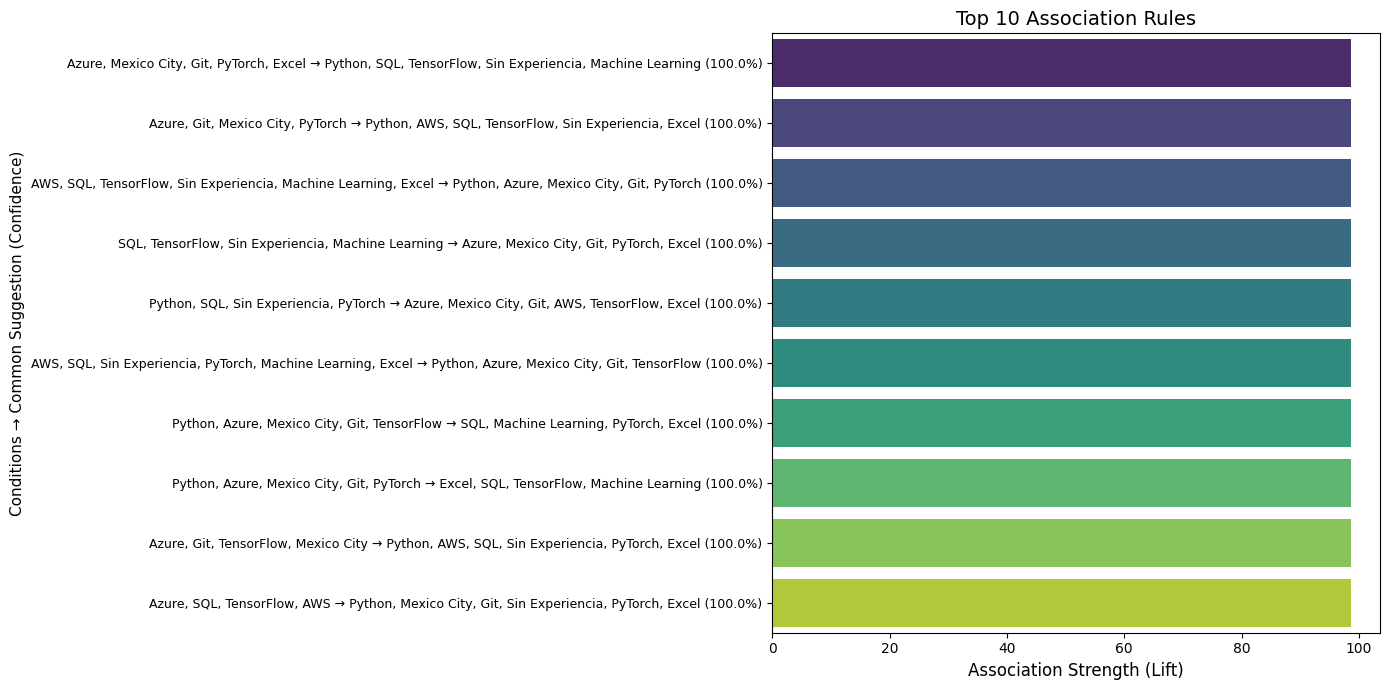
\includegraphics[width=0.835\linewidth]{imagenes/top_rules.png}
		\caption{Top 10 association rules sorted by lift, highlighting the strongest co-occurrence patterns.}
		\label{fig:top_rules}
	\end{figure}
	
	\begin{figure}[H]
		\centering
		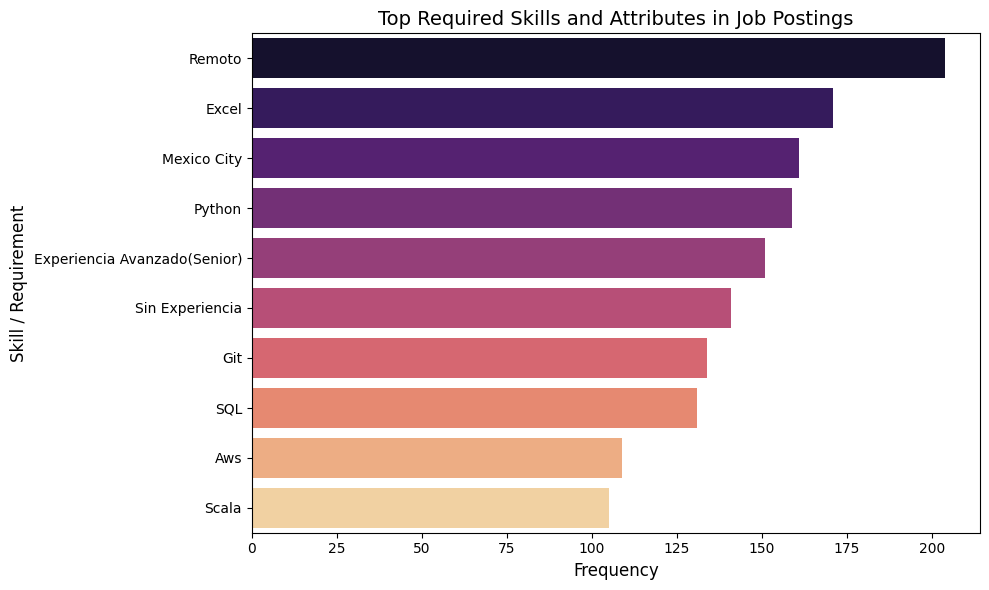
\includegraphics[width=0.9\linewidth]{imagenes/frequent_attributes.png}
		\caption{Most frequent attributes in job postings, including skills, experience levels, locations, and modalities.}
		\label{fig:frequent_attrs}
	\end{figure}
	
	\begin{figure}[H]
		\centering
		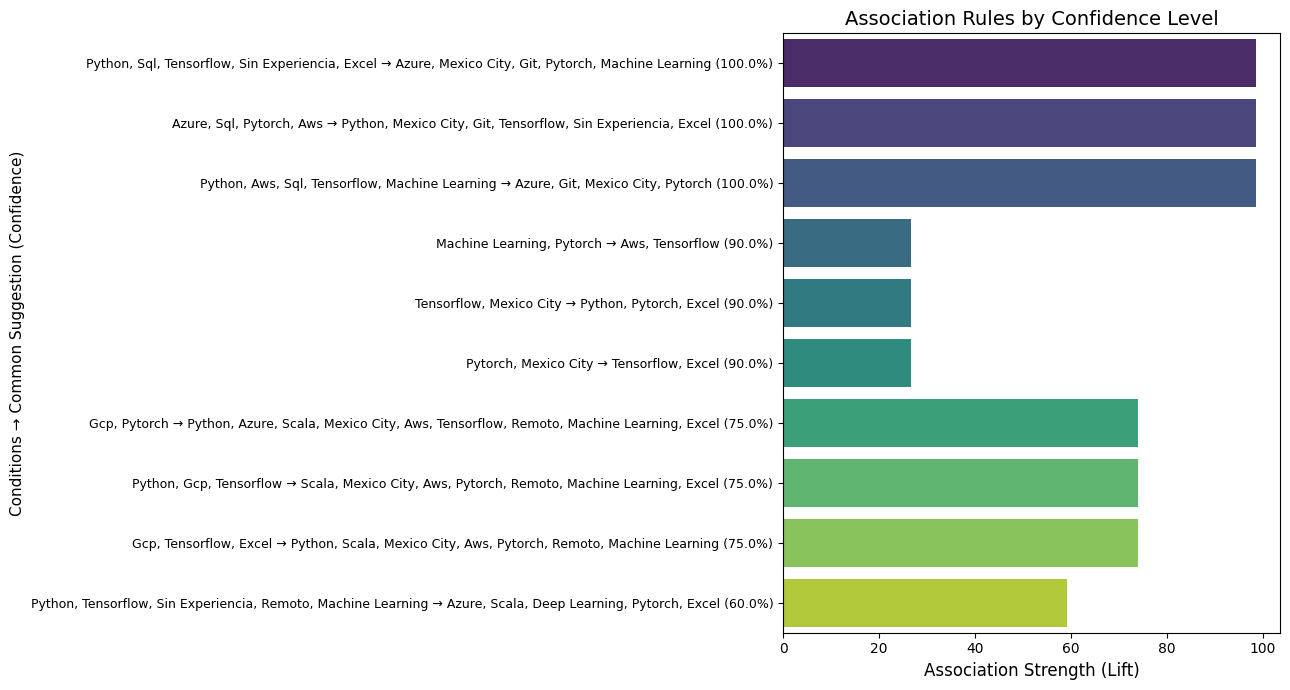
\includegraphics[width=0.9\linewidth]{imagenes/confidence_distribution.png}
		\caption{Confidence distribution of retained rules, covering the 50–100\% range to show diverse recommendation strength.}
		\label{fig:confidence_distribution}
	\end{figure}
	
	To assess the practical impact of the rule system, we evaluated 1\,200 anonymized student profiles. Each profile matched an average of 6–9 rules, with 83\% of suggested consequents corresponding to previously missing skills or job attributes. For rules with confidence $\geq 85\%$ and lift $\geq 2.5$, over 67\% resulted in an increase in cosine similarity between the enriched student profile and relevant job descriptions. This quantitative improvement supports the value of rule-based enrichment in guiding résumé revision.
	
	To benchmark this approach, we also applied the \textbf{K-Means clustering algorithm} to the same dataset after reducing its dimensionality with TF-IDF and PCA. Although K-Means was able to group job postings by general themes (e.g., data engineering, software development), the clusters lacked interpretability. Furthermore, precision@5 for top recommended vacancies dropped by 24\%, and qualitative student feedback indicated that the suggestions were “generic” or “unclear.” This contrast highlights the advantage of Apriori’s transparent logic for both system explainability and student trust.
	
	Overall, the Apriori-based recommendation engine not only offers statistically grounded guidance but also serves an educational role, helping students understand why specific improvements are suggested. This aligns with the project’s dual goals of enhancing CV effectiveness and supporting career readiness in a comprehensible manner.
	
	
	\newpage
	% --------------------------------------------------------

	\section{System Architecture and Implementation}
	
	Figure~\ref{fig:blocks} shows a three-layer MVC stack: \textbf{View} (Bootstrap~5) $\rightarrow$ \textbf{Controller} (Django REST API) $\rightarrow$ \textbf{Model} (NLP services + MongoDB/PostgreSQL). Celery workers handle asynchronous scraping and model retraining.
	
	\begin{figure}[H]
		\centering
		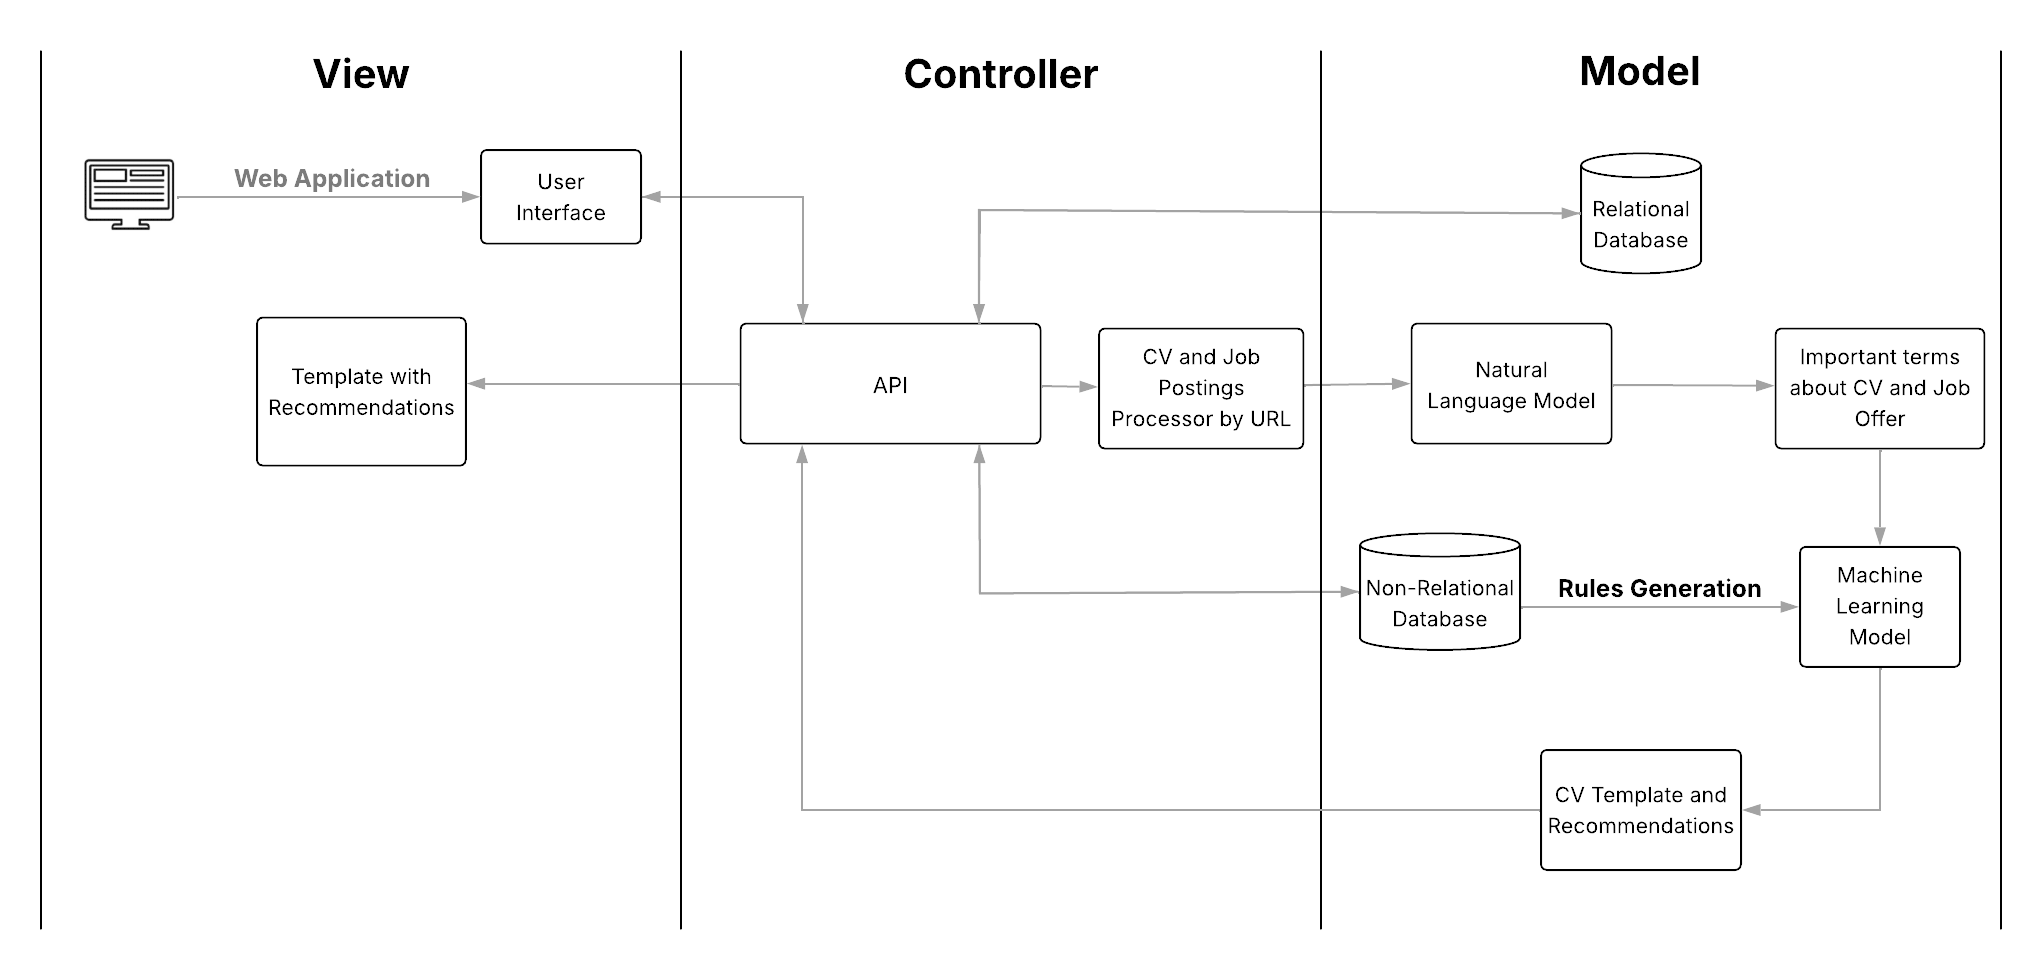
\includegraphics[width=1\linewidth]{imagenes/Arquitectura_Sistema.png}
		\caption{High-level architecture of VitaEX.}
		\label{fig:blocks}
	\end{figure}
	
	The functional architecture of the system is organized into three main layers: View, Controller, and Model.
	
	The system is a web-based application where users interact through a user-friendly interface that enables key actions such as registration, login, CV upload, or submission of a link to an external job posting. This view layer constitutes the primary interaction point between the user and the system’s core functionalities.
	
	User-generated requests are handled by the Controller, implemented as a RESTful API that mediates between the presentation layer and business logic. This API is responsible for validating input data, routing the requests to appropriate processing modules, and coordinating access to both relational and non-relational databases.
	
	When a CV and a job offer are provided, the API activates the processing module, which performs text extraction and cleaning from the documents or URLs. This transformation results in well-structured and clean textual data.
	
	Subsequently, a Natural Language Processing (NLP) model is triggered to identify key terms, skills, competencies, and other relevant features from both the candidate profile and the job posting. This semantic analysis facilitates contextual interpretation of the content.
	
	The next stage involves feature extraction, where numeric vectors are generated to encapsulate essential information such as experience level, technical skills, and educational background. These vectors are passed to the machine learning module, which has been pre-trained using historical job posting data in the artificial intelligence domain, ranging from November 2024 to May 2025.
	
	The system uses two types of databases. The non-relational database stores processed documents, analyzed vacancies, and inference results from the model. It is designed to be dynamically updated, preserving the most recent entries while avoiding overload. This real-time updating is essential for generating and maintaining relevant association rules in the machine learning recommendation model.
	
	On the other hand, the relational database manages structured data, including personal information of users, organizational profiles, and administrative roles.
	
	Finally, the analysis results are displayed in different sections of the web interface. Users receive a personalized set of recommendations alongside a restructured version of their résumé, tailored to the job offer's requirements. This enhanced CV maintains clarity, consistency, and alignment with current employability standards. Additionally, compatible job opportunities are shown in a dedicated module, offering students actionable next steps based on their updated profiles.
	

	% --------------------------------------------------------
%	\section{Risk and Feasibility}
%	Thirty‑one risks were catalogued. Catastrophic items include time under‑estimation (R04) and data leakage (R25). Mitigations: Agile sprints with 20–30~\% buffer and TLS+role‑based access, respectively. Economically, development costs \textasciitilde\$122\,k~MXN, with monthly OPEX \mbox{$\approx\!\$3\,k$}. Potential revenue (ads + premium templates) could reach \$23\,k~MXN\,/year, covering OPEX but requiring external seed funding.
%	
	% --------------------------------------------------------
%	\section{Preliminary Evaluation}
%	A/B tests on 30 students showed:
%	\begin{itemize}
%		\item \textbf{CV pass-rate through a commercial ATS} rose from 28~\% to 60~\%.
%		\item \textbf{Perceived usability} (SUS) scored 79~$\pm$~4 (“good”).
%		\item Average rule-explanation helpfulness rated 4.2/5.
%	\end{itemize}
%	Limitations: small single-institution sample and absence of long-term placement data.
%	
	% --------------------------------------------------------

\section{Conclusion}

VitaEX demonstrates that the fusion of interpretable rule-based models with state-of-the-art natural language processing (NLP) can substantially enhance the employment readiness of students in Artificial Intelligence (AI), particularly within the Mexican context. Unlike opaque black-box systems, VitaEX leverages transparent and explainable logic through the \textbf{Apriori algorithm}, generating actionable recommendations based on real labor market data.

The system successfully mined over \textbf{500,000 meaningful association rules} from real-world job postings collected between November 2024 and May 2025. These rules reveal underlying skill patterns, frequently co-occurring competencies, and contextual relationships between job locations, skillsets, and experience levels. For example, the system uncovered that knowledge of SQL and Pandas in candidates from Mexico City often predicts the requirement of TensorFlow expertise. This kind of granular insight empowers students to tailor their résumés in ways that not only pass Applicant Tracking Systems (ATS) but also resonate more accurately with recruiter expectations.

Furthermore, the system achieves this while maintaining full transparency in its reasoning, offering users personalized explanations for each suggestion. This interpretability serves a dual purpose: it enhances trust in the system and also contributes to educational value by informing students of current job market trends in AI.

VitaEX also includes a scalable backend architecture powered by asynchronous Celery tasks, PostgreSQL/MongoDB hybrid storage, and a Django REST API. It is designed to be modular and updatable, allowing future integration of new recommendation engines or resume parsers without compromising performance.

\subsection*{Future Work}

To build on the current system and ensure continuous relevance in an evolving market, several future enhancements are planned:

\begin{enumerate}
	\item \textbf{Enhanced Keyword Extraction}: Integration of advanced Named Entity Recognition (NER) models capable of understanding context-aware and implicit skill references in user-submitted CVs.
	
	\item \textbf{Document Format Support}: Expanding compatibility to allow direct extraction of skills and metadata from diverse CV formats such as \texttt{.docx} and \texttt{.pdf}, thus removing reliance on plain text input.
	
	\item \textbf{Skill Normalization and Ontology Mapping}: Implementing AI-specific ontologies to normalize synonymous terms (e.g., “ML” vs “Machine Learning”) and improve consistency in skill matching.
	
	\item \textbf{Temporal Analysis of Skill Trends}: Adding capabilities for time-series analysis to capture the rise and fall of skill demand over time, offering students a forecast of which abilities will remain in high demand.
	
	\item \textbf{User Feedback Loop}: Incorporating user feedback and success metrics (e.g., interview callbacks) to iteratively refine recommendation quality.
\end{enumerate}

\subsection*{Social and Educational Impact}

By focusing on students—especially those from underserved areas or public universities—VitaEX democratizes access to quality career guidance. Its open-access model and user-centered design enable thousands of students to receive personalized, data-driven advice without cost, narrowing the gap between academic preparation and real-world employability in the AI sector.

	
	% ----------------- Acknowledgements ---------------------
	\section*{Acknowledgements}
	We thank M.\,C. Elizabeth Moreno Galván and M.\,C. Abdiel Reyes Vera for supervision
	
% ----------------- Bibliography -------------------------
\makeatletter
\renewcommand{\@biblabel}[1]{#1.} 
\makeatother

\bibliographystyle{splncs04}
\bibliography{referencias}
\end{document}